\documentclass[10pt, a4paper]{article}
\usepackage{a4wide}

\usepackage[ngerman]{babel}
\usepackage[utf8]{inputenc}
\usepackage[T1]{fontenc}

\usepackage{parskip}
\usepackage{graphicx}

\newcommand{\ra}{$\rightarrow$ }
\newcommand{\Ra}{$\Rightarrow$ }
\newcommand{\la}{$\leftarrow$ }
\newcommand{\La}{$\Leftarrow$ }

\newcommand{\delt}{\mathrm{d}}

\setcounter{section}{-1}

\title{Gerätekonstruktion WS 16/17}


\begin{document}

\maketitle
\tableofcontents

\let\thefootnote\relax\footnotetext{Anmerkungen:}
\let\thefootnote\relax\footnotetext{- Fehlerfunde bitte an s75662@htw-dresden.de schicken, danke :)}
\let\thefootnote\relax\footnotetext{- Vorhandene handschriftliche Grafiken sind Platzhalter und werden in naher Zukunft noch digitalisiert.}

\newpage

\section{Organisatorisches}
Prof. Bauer, Raum Z442 (440, 431)

Modul besteht aus den Units Gerätekonstruktion \emph{und} Werkstofftechnik, d.h. es gibt nur eine Prüfung.

2 GK Praktika im Laufe des Semesters mit je 2 SWS, beginnend KW44.

GK-Übung findet 14-tägig statt.

Skript gibt's im Downloadbereich. Siehe Sidebar rechts auf Prof.-Seite. \\Nutzername: grstudium

Literaturempfehlung: Gerätekonstruktion in der Feinwerktechnik und Elektronik. Siehe Skript für Details.

\section{Einführung in die Gerätekonstruktion}

3 Axiome der Konstruktionswissenschaft

\begin{enumerate}
	\item Ganzheitsaxiom:
		Gesamtes System betrachten, nicht nur Einzelteil
	\item Zeitwertaxiom:
		Jede Entwicklung wird langfristig durch Bessere ersetzt
	\item Fehleraxiom:
		Es gibt immer Abweichungen zu beachten
\end{enumerate}

$\Rightarrow$ Ein Produkt hat Bestand am Markt, wenn es Kunden einen sinnvollen und anwendungsgerechten Nutzen für die geplante Nutzungsdauer zu einem bezahlbaren Preis bietet. (realisierter Gebrauchswert)

\section{Systembetrachtung elektronischer und elektromechanischer Geräte}
\subsection{Funktionsstrukturen}

\underbar{a) Allgemeines Modell eines technischen Systems}

\begin{center}
	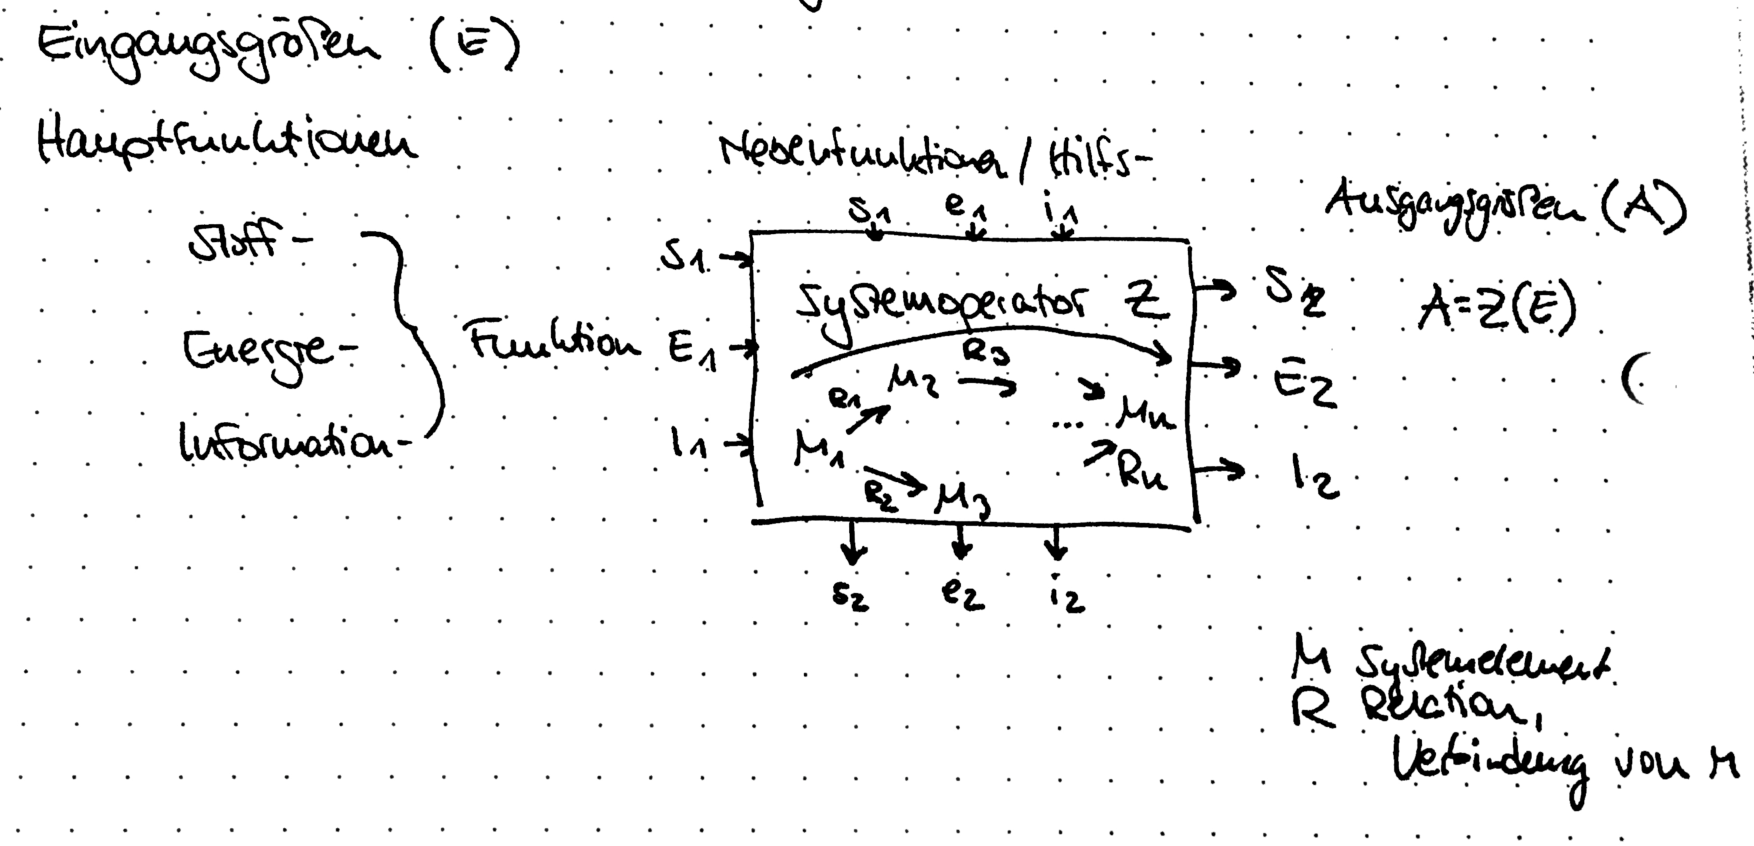
\includegraphics[width=.8\textwidth]{img/1_1}
\end{center}

\underbar{b) Allgemeines Gerätemodell}

\begin{minipage}{.3\textwidth}
	Betrachtungsebene\\ funktioneller Struktur
	\begin{itemize}
		\item \underbar{Kommunikationsebene}\\
			Stoff-, Energie- und Informationsaustausch zwischen Mensch und Gerät oder Gerät und Gerät
		\item \underbar{Verarbeitungsebene}\\
			Art und Weise der definierten Verarbeitung von Eingangsgrößen zu Ausgangsgrößen
		\item \underbar{Störgrößenebene}\\
			Maßnahmen zur Sicherung der Gerätefunktion und zum Schutz gegen Einwirkungen von außen und nach außen
	\end{itemize}
\end{minipage}
\begin{minipage}{.3\textwidth}
	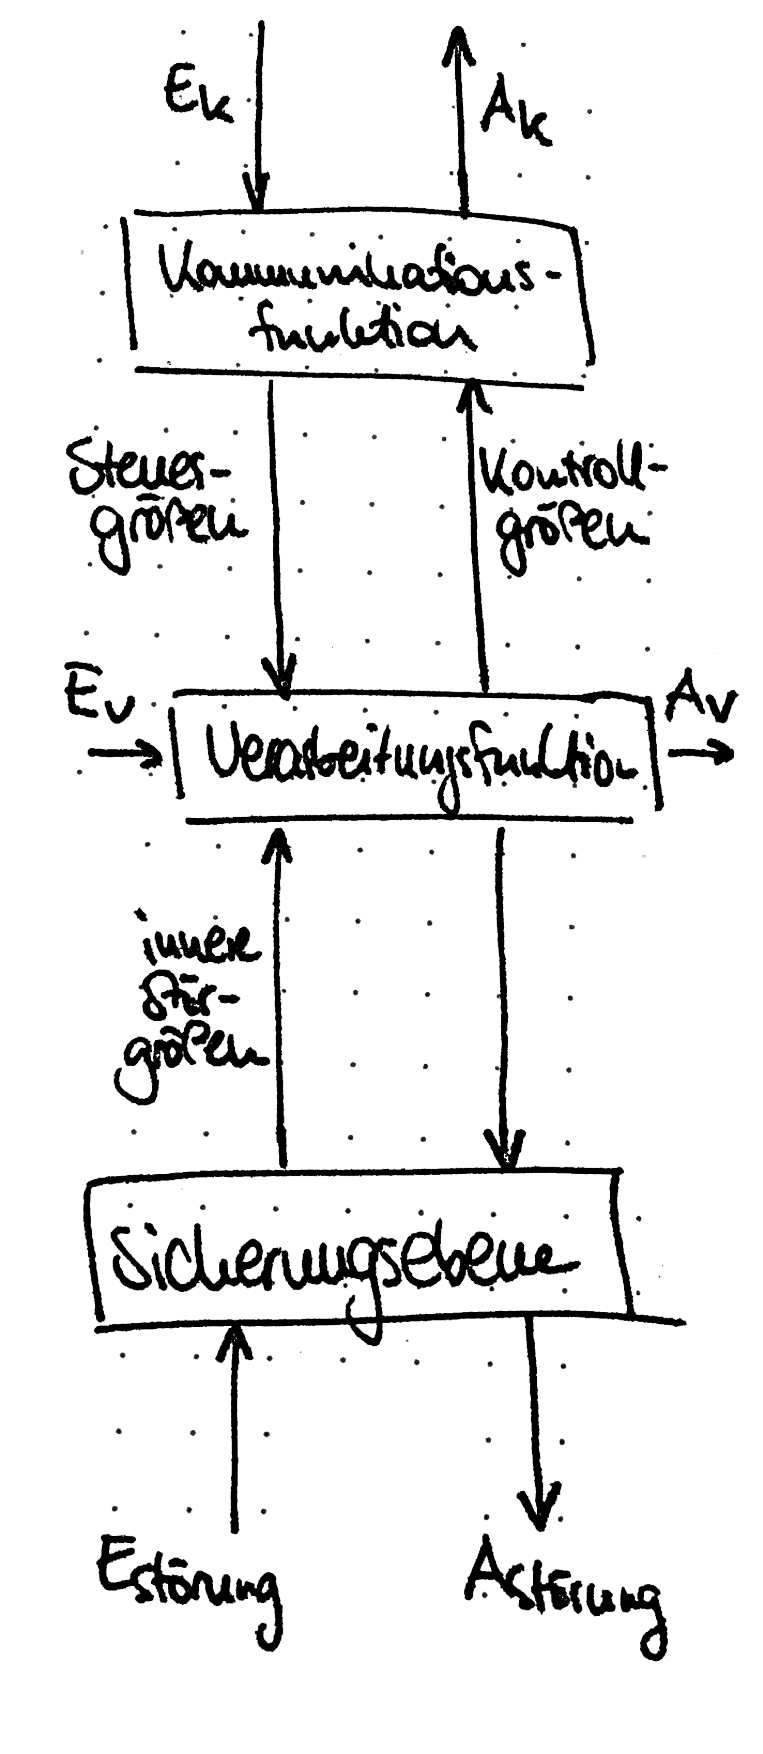
\includegraphics[width=\textwidth]{img/2_1}
\end{minipage}
\begin{minipage}{.3\textwidth}
	Betrachtungsebene geometrisch-stofflicher\\ Struktur
	\begin{itemize}
		\item Bedien- und Anzeigeelemente\\ (z.B. Tasten, Monitor)
		\item Interfaceelemente\\ (z.B. Stecker, Buchsen, mechanische Verbindungen)
		\item Bauelemente zur Realisierung der Verarbeitungsfunktion\\ (z.B. IC (Integrierter Schaltkreis), Transistor, Welle)
		\item Bauelemente zur Stützfunktion\\ (z.B. Gestell, Träger)
		\item Bauelemente zur Schutzfunktion\\ (z.B. Gehäuse, Umhüllung, Abschirmung, Wärmeabführung)
	\end{itemize}
\end{minipage}

\Ra vgl. erweitertes allgemeines Gerätemodell mit Softwareanteil <Folie 36>

\subsection{Hierarchieebenen der Gerätegestaltung}

\underbar{a) Hierarchieebenen der Funktionselemente}

\begin{tabular}{p{.3\textwidth} p{.3\textwidth} p{.3\textwidth}}
\hline
Funktionsschicht/\newline Wirkfläche & sind die am Funktionsfluss direkt beteiligten Oberflächen, Geometrien, Schichten mit entsprechenden werkstofflichen Eigenschaften & z.B. Widerstandsschicht\\ \hline
Einzelteil & niedrigste Ebene der körperlichen Zerlegung eines Geräts, bestimmt durch Werkstoff und Geometrie & z.B. Zahnrad, Widerstandsbauelement\\ \hline
Baugruppe & abgegrenzte, selbständige Gruppe von Einzelteilen, die miteinander verkoppelt sind und eine prüfbare Teilfunktion realisieren & z.B. Leiterplattenbaugruppe, Getriebe\\ \hline
\end{tabular}

\begin{tabular}{p{.3\textwidth} p{.3\textwidth} p{.3\textwidth}}
\hline
Einzelgerät & aus Baugruppen und Einzelteilen zusammengesetztes System mit einer Gesamtfunktion & z.B. Zählwerk, Messgerät, Netzteil\\ \hline
Anlage & Erfüllung komplexer, mehrerer Funktionen durch Verknüpfung von mehreren Geräten & z.B. Messplatz, Automatisierungsanlage\\ \hline
\end{tabular}

\vspace{1cm}
\underbar{\textbf{Beachte:}}

\begin{tabular}{p{.3\textwidth} p{.3\textwidth} p{.3\textwidth}}
\hline
Bauelement & werden bei der Betrachtung nicht weiter zerlegt und können Einzelteil oder Baugruppe sein & z.B. Widerstandsbauelement, gehäustes Halbleiterbauelement\\ \hline
\end{tabular}

\vspace{1cm}
\underbar{b) Hierarchieebenen der Verbindungen und Verdrahtungen}

Nutzung von Verbindungen und Verdrahtungen (elektronische und elektrische Verbindungen) zur Realisierung der nächsthöheren Hierarchieebene der Funktionselemente.

z.B.

\begin{itemize}
	\item interne Bauelementeverdrahtung
	\item Verbindung auf dem Verdrahtungsträger zur elektronischen Baugruppe
	\item interne Geräteverdrahtung zwischen den Baugruppen
	\item Geräteverdrahtung als externe Verbindung zwischen Geräten zu einer Anlage
\end{itemize}

\end{document}